\documentclass{beamer}
\usetheme{Boadilla}
\usepackage{tikz}
% \usepackage{enumitem}

\title{MTH 1020 Week 9 tutorial}
\author{Alex Elzenaar}

\newcommand{\R}{\mathbb{R}}

\begin{document}
\begin{frame}{\inserttitle}
\begin{enumerate}
  \item Feedback on A2
  \item A work through of an A2 question
  \item Reminder of continuity etc
  \item Problem sheets!
\end{enumerate}
\end{frame}


\begin{frame}{Feedback on Asst. 2}

  \begin{itemize}
    \item \textbf{Please scan or use a `PDF scanner' on your phone rather than the camera.} If what you write is not readable because of blur or shadows then you will lose marks.
    \item Many people had trouble with the question `if two planes are not parallel then they intersect in a line''. People reverted to vague arguments about `curves' (what is a curve?)
          or `flatness' or tried to use some notion of `dimension' (which we have not done in this course, so just like in A1 where people tried to use calculus to prove an inequality
          it should be a hint that you are doing the wrong thing).
    \item In Q5, many people stated an answer without any proof.
  \end{itemize}

\end{frame}


\begin{frame}

\begin{theorem}
  If $ P $ and $ Q $ are two non-parallel planes in $ \R^3 $, then they intersect in a line.
\end{theorem}

\begin{enumerate}
  \item Let $ P $ and $ Q $ be planes that are not parallel.
  \item Without loss of generality, we can assume $P$ is the $ xy$-plane (why?). This means that $ P $ and $ Q $ have equations
        \begin{gather*}
          P = \{ (x,y,z) \in \R^3 : z = 0 \}\\
          Q = \{ (x,y,z) \in \R^3 : n_1 x + n_2 y + n_3 z = b \}.
        \end{gather*}
        where $ \vec{n} = (n_1,n_2,n_3) $ is a nonzero vector orthogonal to $ Q $, and $ b \in \R $.
  \item Since $ P $ and $ Q $ are not parallel, it cannot be that $ \vec{n} = (0,0,n_3) $: one of $ n_1 $ or $ n_2 $ is non-zero. We proceed in two cases; the first case is
        that $ n_1 \neq 0 $ (the case for $ n_2 \neq 0 $ is very similar).
\end{enumerate}
\end{frame}




\begin{frame}

\begin{block}{Standing assumptions}
Standing assumptions: planes are $ P = \{ (x,y,z) \in \R^3 : z = 0 \} $, $Q = \{ (x,y,z) \in \R^3 : n_1 x + n_2 y + n_3 z = b \} $; $ n_1 \neq 0 $.
\end{block}

\textbf{Suppose that} $ \vec{v} = (x,y,z) \in P \cap Q $.
\begin{enumerate}
  \item Since $ \vec{v} \in P $, $ z = 0 $. Since $ \vec{v} \in Q $, $ b = n_1 x + n_2 y $.
        Since $ n_1 \neq 0 $, $ x = (n_2 y - b)/n_1 $.
  \item Therefore,
  \begin{displaymath}
    \vec{v} = \left( \frac{b - n_2 y }{n_1}, y, 0 \right) = \left( \frac{b}{n_1}, 0, 0 \right) + y \left( -\frac{n_2}{n_1}, 1, 0 \right).
  \end{displaymath}
  \item Let $ L $ be the line
  \begin{displaymath}
    L = \left\{ \left( \frac{b}{n_1}, 0, 0 \right) + t \left( -\frac{n_2}{n_1}, 1, 0 \right) : t \in \R \right\}.
  \end{displaymath}
  We just showed that if $ \vec{v} \in P \cap Q $, then $ \vec{v} \in L $; i.e. $ P \cap Q \subset L $.
\end{enumerate}
\end{frame}

\begin{frame}
\begin{block}{Standing assumptions}
Planes are $ P = \{ (x,y,z) \in \R^3 : z = 0 \} $, $Q = \{ (x,y,z) \in \R^3 : n_1 x + n_2 y + n_3 z = b \} $; $ n_1 \neq 0 $.
\end{block}

\begin{block}{Previous slide}
We defined  $   L = \left\{ \left( \frac{b}{n_1}, 0, 0 \right) + t \left( -\frac{n_2}{n_1}, 1, 0 \right) : t \in \R \right\} $
and showed that $ P \cap Q \subset L $.
\end{block}

\textbf{We will now show} that $ L \subset P \cap Q $.
\begin{enumerate}
  \item Every element of $ L $ lies in $ P $, since the $ z$-ordinate of every point in $ L $ is $0$.
  \item Also, if $ t \in \R $, then
  \begin{displaymath}
    \frac{b}{n_1} n_1 - t\frac{n_2}{n_1} n_1 + t n_2 + 0 n_3 = b -t n_2 + t n_2 = b:
  \end{displaymath}
  i.e. every point of $ L $ satisfies the equation for $ Q $ in (2), and so $ L \subset Q $.
  \item Therefore $ L \subset P \cap Q $.
\end{enumerate}
\end{frame}


\begin{frame}

\begin{theorem}
  If $ P $ and $ Q $ are two non-parallel planes in $ \R^3 $, then they intersect in a line.
\end{theorem}

\begin{proof}
  We just showed that if $ n_1 \neq 0 $ and $ L $ is the line
  \begin{displaymath}
    L = \left\{ \left( \frac{b}{n_1}, 0, 0 \right) + t \left( -\frac{n_2}{n_1}, 1, 0 \right) : t \in \R \right\}.
  \end{displaymath}
  then $ L \subset P\cap Q $, and $ P \cap Q \subset L $. So $ P \cap Q = L $.

  The case $ n_2 \neq 0 $ is essentially the same but you get
  \begin{displaymath}
    L = \left\{ \left( \frac{b}{n_2}, 0, 0 \right) + t \left(1,  -\frac{n_1}{n_2}, 0 \right) : t \in \R \right\}.
  \end{displaymath}
\end{proof}
\end{frame}


\section{Continuity and differentiability}

\begin{frame}
\begin{theorem}
  The function $ f : \R \to \R $ defined by
  \begin{displaymath} f(x) = \begin{cases} x \sin \frac{1}{x} & x \neq 0\\ 0 & x = 0 \end{cases} \end{displaymath}
  is continuous everywhere on $ \R $ but not differentiable at $ x = 0 $.
\end{theorem}
\begin{proof}[Proof of continuity]
  Since $ x $ and $ \sin(1/x) $ are continuous for all $ x \neq 0 $, their product is continuous for all $ x \neq 0 $. Now observe that, for all $ x $,
  \begin{displaymath}
    -x \leq x \sin (1/x) \leq x.
  \end{displaymath}
  As $ x \to 0 $, $ -x \to 0 $. So $ x \sin (1/x) \to 0 $ (by the \textbf{squeeze theorem}), i.e. $ \lim_{x \to 0} f(x) = 0 = f(0) $.
\end{proof}
\end{frame}

\begin{frame}
\begin{proof}[Proof of (non)-differentiability]
  When $ x \neq 0 $, we can apply the usual differentiation rules to find $ f'(x) = \sin(1/x) - (1/x)  \cos(1/x) $. We now show that $ f $ is not
  differentiable at $ 0 $. In other words we show that $ \lim_{h \to 0} \frac{f(0+h) - f(0)}{h} $ does not exist. We substitute for $ f $:
  \begin{displaymath}
    \lim_{h \to 0} \frac{f(0+h) - f(0)}{h} = \lim_{h \to 0} \frac{h \sin(1/h) - 0}{h} = \lim_{h \to 0} \sin(1/h).
  \end{displaymath}

  \begin{center}
  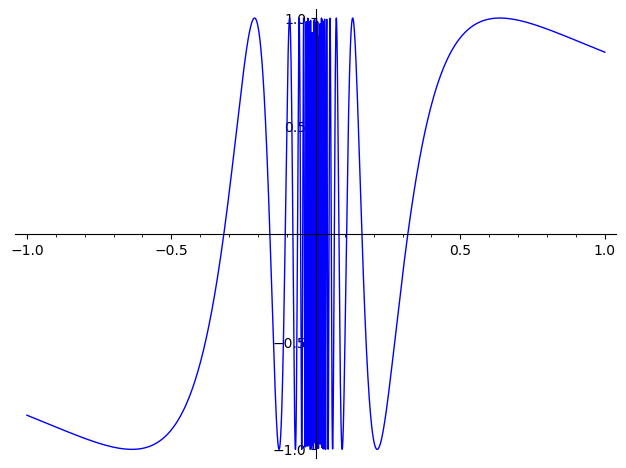
\includegraphics[width=.3\textwidth]{sinx}
  \end{center}

  This limit does not exist, because as $ h \to 0 $ the function $ \sin(1/h) $ oscillates infinitely often between $ \pm 1 $, and does not approach a single value.
\end{proof}
\end{frame}


\begin{frame}{Key concepts so far}
\begin{enumerate}
  \item What is a limit?
  \item \textbf{Definitions:} continuity, differentiability
  \item Usual differentiation laws (chain and product laws, implicit differentiation) and derivatives of basic functions ($ x^n $, $ \sin x $, $ \cos x  $, $ \exp x $, $ \log x $, $ \lvert x \rvert $)
  \item \textbf{Intermediate value theorem:} if $ f : [a,b] \to \R $ is a function, $ f(a) < 0 $, and $ f(b) > 0 $, then there exists $ c \in [a,b] $ such that $ f(c) = 0 $
  \item Extrema: definition of critical point, inflection point, concavity.
\end{enumerate}
\end{frame}



\begin{frame}{\inserttitle}
\begin{enumerate}
  \item Get into groups of 3-4 people who all prepared a different question in advance.
  \item Write your \textbf{preferred name} and \textbf{ID number} on the whiteboards so I can take attendance
  \item Present your prepared question to each other as I come around, you should only take about 5min each for this.
  \item Then get started on the other questions \textbf{in your groups}.
  \item \textbf{At the end:} please erase the boards and return any markers etc that you used (you do not need to return the handouts)
\end{enumerate}
\end{frame}



\end{document}
